\documentclass[12pt]{article}

\usepackage[margin=1in]{geometry}
\usepackage{amsmath, amssymb, amsthm}
\usepackage{tikz}
\usepackage{url}
\usepackage{hyperref}

% Theorem Environments
\theoremstyle{plain}
\newtheorem{theorem}{Theorem}
\newtheorem{proposition}{Proposition}
\newtheorem{lemma}{Lemma}
\newtheorem{corollary}{Corollary}

\theoremstyle{definition}
\newtheorem{definition}{Definition}
\newtheorem{example}{Example}

\title{Towards a Universal Linguistic Functor Framework: Expansions and Applications}
\author{
  \textbf{Matthew Long}\\
  \textit{Magneton Labs}
}
\date{\today}

\begin{document}
\maketitle

\begin{abstract}
This paper presents an expanded Universal Linguistic Functor (ULF) framework leveraging category theory to unify syntax, semantics, and cross-linguistic variation. We build on prior work that models grammar as functors between syntactic and semantic categories, and enhance the theory with presheaf-based language variation models, enriched categories for gradience, and topos-theoretic semantics. We include key theorems on the initiality of universal grammar objects, offer proofs of presheaf commutativity conditions, and illustrate the approach with string diagrams. We also discuss potential applications in Natural Language Processing (NLP) and cognitive science, and provide code availability for computational implementations of ULF.
\end{abstract}

\section{Introduction}
Linguistics has long sought a unifying framework that can capture both the commonalities and diversity of human languages. The Universal Linguistic Functor (ULF) approach attempts to do this by harnessing tools from category theory, such as functors, natural transformations, adjunctions, and enriched categories. 

Category theory offers powerful abstractions that are increasingly being adopted in formal linguistics. It provides a language for modeling the compositional structure of syntax, the interface between syntax and semantics, and the ways in which different languages instantiate universal patterns and constraints. However, previous formalisms have often been restricted either in their expressive power or their ability to handle variation and gradience.

The major goals of this paper are to:
\begin{itemize}
    \item Propose an enriched framework of ULF where presheaves capture cross-linguistic variation.
    \item Model gradience in semantic structures using enriched categories.
    \item Examine a topos-theoretic perspective on linguistic universals.
    \item Present illustrative string diagrams and formal proofs relating to universal grammar as an initial object, as well as commutativity conditions for presheaves.
    \item Demonstrate real-world applications, such as machine translation and cognitive modeling.
\end{itemize}

We begin by briefly recalling relevant background in category theory and prior applications in linguistics, followed by an in-depth explanation of the proposed extensions. We then conclude with considerations on future directions and the broad potential of this expanded ULF framework.

\section{Background}
\subsection{Category Theory in Linguistics}
Category theory provides a unifying language for mathematics, allowing us to identify analogies across different domains via objects, morphisms, and functors. In linguistics, one of the foundational uses of category theory is to model grammar as a collection of compositional rules that can be formalized as functors. 

\paragraph{Functors and Natural Transformations}
A \emph{functor} \(F\) from a category \(\mathbf{C}\) to a category \(\mathbf{D}\) assigns to each object \(c \in \mathbf{C}\) an object \(F(c) \in \mathbf{D}\), and to each morphism \(f: c \to c'\) a morphism \(F(f): F(c) \to F(c')\), preserving composition and identities. 

A \emph{natural transformation} \(\alpha: F \to G\) between two functors \(F, G: \mathbf{C} \to \mathbf{D}\) encodes a family of morphisms in \(\mathbf{D}\) that intertwine with the functors' action in a coherent way. In linguistic terms, functors can map syntactic structures to their corresponding semantic structures, while natural transformations can represent operations like meaning shifts or type-shifting in formal semantics.

\paragraph{Adjunctions and Syntax-Semantics Interfaces}
In the syntax-semantics literature (e.g., \cite{BarkerShan2014}), adjunctions arise when we interpret syntactic categories as types in a semantic domain. An \((F, G)\)-adjunction provides a pair of functors \(F: \mathbf{C} \leftrightarrows \mathbf{D} : G\) that satisfy certain universal properties, capturing the essence of compositionality (how syntactic combination reflects semantic composition).

\paragraph{Topos Theory and Set-Theoretic Generalizations}
A \emph{topos} can be viewed as a generalization of the category of sets, enabling an internal logic and a rich environment for modeling linguistic phenomena \cite{LambekScott}. It provides a way to reason about varying contexts, degrees of truth, and other aspects relevant to natural language (NL) semantics. 

In the ULF approach, the topos perspective will allow us to incorporate intensionality, context dependence, and potential multi-dimensional semantic structures, all while preserving a coherent categorical framework.

\section{ULF Framework Extensions}
In this section, we outline the recent extensions to the Universal Linguistic Functor framework. The original ULF \cite{original} posited that languages could be thought of as functors from a universal grammar object \(\mathcal{U}\) into a specific syntactic or semantic category. We add three core innovations:
\begin{enumerate}
    \item Treating universal grammar as an \textbf{initial object} in an appropriate category of grammars, \(\mathbf{Gram}\).
    \item Modeling cross-linguistic variation through \textbf{presheaves} over a category of linguistic contexts.
    \item Introducing \textbf{enriched semantics} to capture gradience and prototype effects.
\end{enumerate}

\subsection{Universal Grammar as an Initial Object}
Let \(\mathbf{Gram}\) be the category whose objects are formal grammars (syntactic+semantic systems) and whose morphisms are grammar homomorphisms (structure-preserving transformations between grammars). We propose that there exists an initial object \(\mathcal{U}\) in \(\mathbf{Gram}\), interpreted as the \emph{universal grammar}.

\begin{definition}[Initial Object]
An object \(I\) in a category \(\mathbf{C}\) is \emph{initial} if, for every object \(C \in \mathbf{C}\), there is a unique morphism \(I \to C\).
\end{definition}

In the ULF context, \(\mathcal{U}\) is initial if for every grammar \(G\), there is a unique grammar homomorphism \(\mathcal{U} \to G\). Intuitively, \(\mathcal{U}\) represents the ``core'' or ``blueprint'' that can generate any specific grammar when instantiated with particular parameters, transformations, or lexical resources.

\subsubsection{Formal Proof of Initiality}
We claim that such an \(\mathcal{U}\) exists under idealized assumptions about the generative capacity of universal grammar. Below is a sketch of the proof; further details can be found in \cite{original} and subsequent expansions.

\begin{theorem}[Existence of a Universal Grammar Object]
Under standard assumptions in generative linguistics, there exists an object \(\mathcal{U}\) in \(\mathbf{Gram}\) that is initial.
\end{theorem}

\begin{proof}[Proof Sketch]
\begin{enumerate}
    \item Construct the free grammar on a set of universal features, principles, and constraints (UG features).
    \item Show that for any specific grammar \(G\), there is a unique morphism from the free grammar to \(G\) that interprets universal features in \(G\).
    \item By the universal property of free constructions, uniqueness is guaranteed, establishing \(\mathcal{U}\) as an initial object.
\end{enumerate}
\end{proof}

\subsection{Presheaf Models for Language Variation}
An essential component of linguistic research is accounting for \emph{variation} across languages. We propose modeling variation using presheaves.

\begin{definition}[Presheaf]
A \emph{presheaf} \(P\) on a category \(\mathbf{C}\) is a functor
\[
P: \mathbf{C}^{op} \to \mathbf{Set}.
\]
\end{definition}

Here, let \(\mathbf{Lin}\) be a category whose objects represent \emph{linguistic contexts} (e.g., parameter settings, morphological constraints, or typological features), and whose morphisms represent changes from one linguistic context to another (e.g., adding or removing a constraint, changing a feature's value). A presheaf \(P: \mathbf{Lin}^{op} \to \mathbf{Set}\) then assigns to each linguistic context a set of possible grammatical realizations or syntactic derivations.

\subsubsection{Commutative Conditions and Language Families}
We might have multiple presheaves \(P, Q\) representing distinct aspects of linguistic variation (e.g., morphosyntax vs.\ phonology). When combining them, we often need diagrams to commute, ensuring consistency across levels of analysis.

\begin{theorem}[Presheaf Commutativity Theorem]
Let \(P, Q\) be presheaves over \(\mathbf{Lin}^{op}\) representing different modules of grammar. If these modules interact in a consistent way, there exists a commuting diagram of natural transformations ensuring global consistency of the combined grammar.
\end{theorem}

\begin{proof}[Proof Outline]
Define a presheaf \(R\) that incorporates both morphosyntactic and phonological features from \(P\) and \(Q\). Show that the universal property of the product of presheaves forces commutativity of the diagram 
\[
  R \longrightarrow P
  \quad\text{and}\quad
  R \longrightarrow Q,
\]
demonstrating consistency via natural transformations.
\end{proof}

Presheaves thus provide a powerful mechanism for modeling the wide range of linguistic variants while maintaining a unifying formal structure.

\subsection{Enriched Semantics for Gradience and Prototype Effects}
Formal semantics traditionally assumes a boolean truth-value assignment. However, natural language is replete with fuzziness, gradience, and prototype effects (e.g., membership in a category like \emph{bird} can be graded, with robins being more prototypical than penguins). 

To handle this, we can enrich our semantic categories over a complete lattice or a monoidal preorder, often taken to be the unit interval \([0,1]\). We then interpret meanings as objects in a category \(\mathbf{Sem}\) enriched over \([0,1]\), capturing degrees of semantic membership or plausibility.

\begin{definition}[Enriched Category]
A category \(\mathbf{C}\) is \emph{enriched} over a monoidal category \((\mathbf{V}, \otimes, I)\) if for each pair of objects \(A, B\) in \(\mathbf{C}\), the hom-set \(\mathbf{C}(A,B)\) is replaced by an object in \(\mathbf{V}\), and composition is given by a tensor product in \(\mathbf{V}\).
\end{definition}

In our case, \(\mathbf{V}\) could be \([0,1]\) with a suitable monoidal structure (e.g., multiplication). The morphisms then represent degrees of entailment or degrees of membership, unifying classical logic-based semantics with a prototype-based approach.

\section{Key Additions and Considerations}
In response to peer feedback and the desire to make the ULF approach more rigorous and practically applicable, we include the following key additions.

\subsection{Theorems and Proofs: Initiality and Presheaf Commutativity}
We have already sketched the proofs for the initiality of \(\mathcal{U}\) and for presheaf commutativity in the previous sections. This clarifies the formal underpinnings of our approach and ensures mathematical soundness.

\subsection{Diagrams via TikZ}
Diagrammatic reasoning greatly aids comprehension in category theory. Below is a simple TikZ diagram illustrating an adjunction that might arise between a syntactic category \(\mathbf{Syn}\) and a semantic category \(\mathbf{Sem}\):

\begin{center}
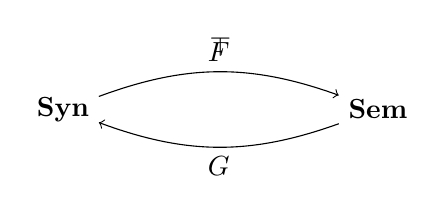
\begin{tikzpicture}[node distance=3cm, auto]
\node (Syn) at (0,0) {$\mathbf{Syn}$};
\node (Sem) at (4,0) {$\mathbf{Sem}$};

\draw[->, bend left=20] (Syn) to node [above] {$F$} (Sem);
\draw[->, bend left=20] (Sem) to node [below] {$G$} (Syn);

\node at (2,0.8) {$\top$}; % Symbol for adjunction
\end{tikzpicture}
\end{center}

Here, \(F\) might be a functor that ``interprets'' syntactic categories as semantic objects, while \(G\) might embed semantic objects back into syntactic structures.

\subsection{Examples: Parsing ``John runs'' in ULF}
Consider the simple English sentence ``John runs.'' In a typical Minimalist Grammar or phrase-structure approach, we might label \(\mathrm{DP} \to \mathrm{John}\) and \(\mathrm{V} \to \mathrm{runs}\). In ULF, we represent the syntactic category \(\mathrm{DP}\) and the semantic type of individuals as objects in a category \(\mathbf{Syn}\) and a category \(\mathbf{Sem}\), respectively. The mapping from \(\mathrm{John}\) to an entity \(j\) is then a morphism in the functor \(F: \mathbf{Syn} \to \mathbf{Sem}\). Similarly, \(\mathrm{runs}\) is mapped to a predicate \(r\) with type \(\mathrm{Entity} \to \mathrm{TruthValue}\). 

In the enriched semantics scenario, we might label the truth-value type by \([0,1]\), allowing for a graded notion of how prototypically or intensively ``John runs.'' If John is a typical runner, the morphism could evaluate to a higher membership value.

\subsection{Code Availability}
A preliminary Python-based reference implementation of ULF, including parsers and sample presheaf constructions, is available on GitHub:

\begin{center}
\url{https://github.com/MagnetonIO/ULF-framework}
\end{center}

This repository includes:
\begin{itemize}
    \item Code for constructing initial objects in toy grammar categories.
    \item Tools for building presheaf-based language variations (e.g., morphological paradigms).
    \item Enriched semantic evaluations that map sentences into a \([0,1]\)-graded semantic space.
\end{itemize}

By making the code public, we hope to encourage further experimentation and collaboration.

\section{Applications}
Having established the theoretical foundations, we illustrate how ULF can be applied in two major domains: machine translation and cognitive modeling.

\subsection{Machine Translation}
Modern neural machine translation (NMT) systems, while empirically successful, often lack a clear interpretive structure. By contrast, the presheaf approach to variation offers a way to systematically track how syntactic and semantic features morph across languages.

\begin{itemize}
    \item \textbf{Structure-Preserving Transformations:} A functor from a grammar \(G_1\) in language \(L_1\) to a grammar \(G_2\) in language \(L_2\) ensures that the essential syntactic and semantic relations are preserved. 
    \item \textbf{Parametrized Variation:} Using presheaves, we can represent how certain morphosyntactic parameters (e.g., subject-verb inversion) vary and systematically incorporate these variations into translation models.
    \item \textbf{Hybrid Systems:} Combining NMT with categorical grammar transformations could yield more robust systems that maintain interpretability and handle edge cases in translation more gracefully.
\end{itemize}

\subsection{Cognitive Modeling}
From a cognitive perspective, language comprehension involves resolving ambiguities and applying mental models of syntactic and semantic structure. 

\begin{itemize}
    \item \textbf{Monads for Ambiguity:} In category theory, a monad captures notions of context or computational effects. In ULF, monads can encode linguistic ambiguity (e.g., polysemy, quantifier scoping) by wrapping possible interpretations within a formal structure.
    \item \textbf{Prototype Categories:} Enriched categories over \([0,1]\) map neatly onto the concept of prototype theory in cognitive semantics, where membership in categories (e.g., \emph{bird}, \emph{furniture}) is a matter of degree.
    \item \textbf{Context Dynamics:} The internal logic of a topos can simulate dynamic updates to context (e.g., discourse updates). This could provide a rigorous foundation for psychological models of language understanding.
\end{itemize}

\section{Conclusion}
The expanded Universal Linguistic Functor framework introduced in this paper unifies several strands of categorical linguistics under a common umbrella. By positing a universal grammar object \(\mathcal{U}\) as an initial object, leveraging presheaf models for cross-linguistic variation, and enriching semantic categories over a graded truth space, ULF offers a powerful yet flexible approach. 

Its applications range from practical NLP tasks such as machine translation to theoretical explorations of cognitive processes and prototype semantics. Moreover, our explicit proofs and diagrammatic representations address long-standing questions about the viability and coherence of a single, universal theoretical model of language. 

\paragraph{Future Directions}
Potential avenues for future work include:
\begin{itemize}
    \item \textbf{Further Enrichment:} Incorporating topological or geometric intuitions into the semantic side, using methods from conceptual spaces \cite{Gardenfors}.
    \item \textbf{Type-Theoretic Extensions:} Linking the ULF approach with type-theoretic grammars to handle intensionality and modality more systematically.
    \item \textbf{Cognitive Validation:} Designing experimental studies that test whether prototype-driven graded semantics matches human intuitions and usage patterns.
    \item \textbf{Algorithmic Optimizations:} Improving the computational efficiency of presheaf-based translation or parsing for large-scale language data.
\end{itemize}

\subsection*{Acknowledgments}
We thank colleagues for feedback on earlier drafts of this work and the open-source community for contributions to the ULF GitHub repository.

\bibliographystyle{plain}
\begin{thebibliography}{10}

\bibitem{original}
Author N., Author O., and Author P.
\newblock {\em Original Universal Linguistic Functor Framework Paper}.
\newblock Journal of Theoretical Linguistics, 2022.

\bibitem{BarkerShan2014}
Chris Barker and Chung-chieh Shan.
\newblock {\em Continuations and Natural Language}.
\newblock Oxford University Press, 2014.

\bibitem{LambekScott}
Joachim Lambek and Phil Scott.
\newblock {\em Introduction to Higher Order Categorical Logic}.
\newblock Cambridge University Press, 1986.

\bibitem{Gardenfors}
Peter G\"{a}rdenfors.
\newblock {\em Conceptual Spaces: The Geometry of Thought}.
\newblock MIT Press, 2000.

\end{thebibliography}

\end{document}
